% ch3p13_001: Using layers: The background rectangles
\documentclass[tikz, border=10pt]{standalone}

\usepackage{tikz}
\usetikzlibrary{arrows.meta, decorations.pathmorphing, backgrounds, positioning, fit, petri}

\begin{document}
	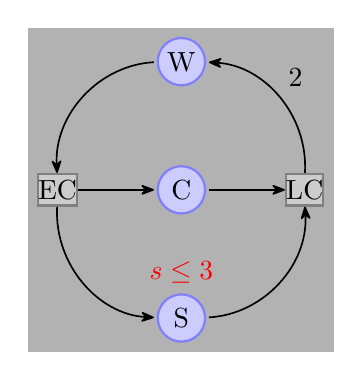
\begin{tikzpicture}[
		place/.style={circle, draw=blue!50, fill=blue!20, thick, inner sep=0pt, minimum size=6mm},
		transition/.style={rectangle, draw=black!50, fill=black!20, thick, inner sep=0pt, minimum size=4mm},
		every label/.style={red},
		bend angle=45,
		pre/.style={<-, shorten >= 1pt, >={Stealth[round]}, semithick},
		post/.style={->, shorten >=1pt, >={Stealth[round]}, semithick}
		]
		\node [place] (waiting) {W};
		\node [place] (critical) [below=of waiting] {C};
		\node [place] (semaphore) [below=of critical, label=above:$s\le 3$] {S};
		
		\node [transition] (leave critical) [right=of critical] {LC}
			edge [pre] (critical)
			edge [post, bend right] node [auto, swap] {2} (waiting)
			edge [pre, bend left] (semaphore);
		
		\node [transition] (enter critical) [left=of critical] {EC}
			edge [post] (critical)
			edge [pre, bend left] (waiting)
			edge [post, bend right] (semaphore);
			
		\begin{scope}[on background layer]
			\node [fill=black!30, fit=(waiting) (critical) (semaphore) (leave critical) (enter critical)] {};
		\end{scope}
	\end{tikzpicture}
\end{document}